\section{Concentration Without Independence}
This chapter mainly explores other approaches to concentration that do not rely on independence.



% ----------5.1----------
\subsection{Cencentration of Lipschitz Functions on the Sphere}
For a random vector $X$ in $\mathbb{R}^n$ and a function $f: \mathbb{R}^n \to \mathbb{R}$. When does the 
random variable $f(X)$ concentrate, i.e.
\[ f(X) \approx \mathbb{E}[f(X)] \text{ with high probability? } \]
If $X$ is normal and $f$ is linear, this is easy: $f(X)$ is normal (\cref{cor:3.3.2}) and concentrates well 
(\cref{prop:2.1.2}).

What about for general \textit{nonlinear} functions $f$? We can't expect good concentration for any $f$, 
but if $f$ does not oscillate too wildly, we might get good concentration. Namely, we'll use Lipschitz 
functions to rule out these oscillations:


\subsubsection{Lipschitz Functions}
\begin{definition}[]
\label{def:5.1.1}
Let $(X, d_X)$ and $(Y, d_Y)$ be metric spaces. A function $f:X \to Y$ is called \underline{Lipschitz} if 
there exists $L \in \mathbb{R}$ such that 
\[ d_Y(f(u), f(v)) \leq L \cdot d_X(u, v) \text{ for every } u, v \in X. \]

The infimum of all $L$ in this definition is called the \underline{Lipschitz norm} because of $f$ and is denoted 
$\lVert f \rVert_{\mathrm{Lip}}$.

If $\lVert f \rVert_{\mathrm{Lip}} \leq 1$, $f$ is called a \underline{contraction}.
\end{definition}

(\textbf{Important}) Technically the Lipschits norm is only a seminorm, since it vanishes on nonzero constant 
functions. It's called a norm in the book for brevity.

The class of Lipschitz functions sits between differentiable and uniformly continuous: 
\[ f \text{ is differentiable } \implies f \text{ is Lipschitz } \implies f \text{ if uniformly continuous.} \]

Moreover, from Exercise 5.1,
\[ \lVert F \rVert_{\mathrm{Lip}} \leq \sup_{x \in \mathbb{R}^n} \lVert \nabla f(x) \rVert_{2}. \]

\begin{example}[]
\label{ex:5.1.2}
Vectors, matries, and norms define natural Lipschitz functions:
\begin{enumerate}
	\item For a fixed vector $\theta \in \mathbb{R}^n$, the linear functional 
	\[ f(x) = \left\langle x, \theta \right\rangle \text{ has Lipschitz norm } 
	\lVert f \rVert_{\mathrm{Lip}} = \lVert \theta \rVert_{2}. \]
	\item More generally, any $m \times n$ matrix $A$, the linear operator 
	\[ f(x) = Ax \text{ has Lipschitz norm } \lVert F \rVert_{\mathrm{Lip}} = \lVert A \rVert_{}. \]
	\item For any norm $\lVert \cdot \rVert_{}$ on $\mathbb{R}^n$, the function 
	\[ f(x) = \lVert x \rVert_{} \]
	has Lipschitz norm equal to the smallest $L$ such that 
	\[ \lVert x \rVert_{} \leq L \lVert x \rVert_{2} \text{ for all } x \in \mathbb{R}^n. \]
\end{enumerate}
\end{example}

\begin{proof}
Exercise 5.2.
\end{proof}


\subsubsection{Concentration via Isoperimetric Inequalities}
Any Lipschitz function on the Euclidean sphere $S^{n - 1} = \{x \in \mathbb{R}^n: \ \lVert x \rVert_{2} = 1\}$ 
concentrates:

\begin{theorem}[]
\label{thm:5.1.3}
Let $X \sim \mathrm{Unif}(\sqrt{n}S^{n - 1})$. Then for any Lipschitz function $f: \sqrt{n}S^{n - 1} \to 
\mathbb{R}$ we have 
\[ \lVert f(X) - \mathbb{E}[f(X)] \rVert_{\psi_2} \leq C \lVert f \rVert_{\mathrm{Lip}}. \]
\end{theorem}

The theorem above works for the geodesic distance metric as well (Exercise 5.4).

\cref{thm:5.1.3} has been proved already for linear functions $f$. \cref{thm:3.4.5} tells us that $X$ is a 
subgaussian random vectos, and this by definition means that any lienar function of $X$ is a subgaussian 
random variable. 

To fully prove \cref{thm:5.1.3}, we need to argue that any Lipschitz function concentrates at least as well 
as a linear function. We'll use the aread of their \underline{sublevel sets} - regions of the sphere where 
$f(x) \leq a$ for a given level $a$. To do this, we'll use the \textit{isoperimetric inequality}, namely 
the one for subsets on $\mathbb{R}^n$: 

\begin{theorem}[Isoperimetric inequality on $\mathbb{R}^n$]
\label{thm:5.1.4}
Among all subsets $A \subset \mathbb{R}^n$ with given volume, the Euclidean balls have minimal area. Moreover, 
for any $\varepsilon > 0$, the Euclidean balls minimize the volume of the $\varepsilon$-neighborhood of $A$, 
defined as 
\[ A_{\varepsilon} = \{ x \in \mathbb{R}^n: \ \exists y \in A \text{ such that } \lVert x - y \rVert_{2} 
\leq \varepsilon \} = A + \varepsilon B_2^n. \] 
The figure below illustrates the isoperimetric inequality:
\begin{center}
	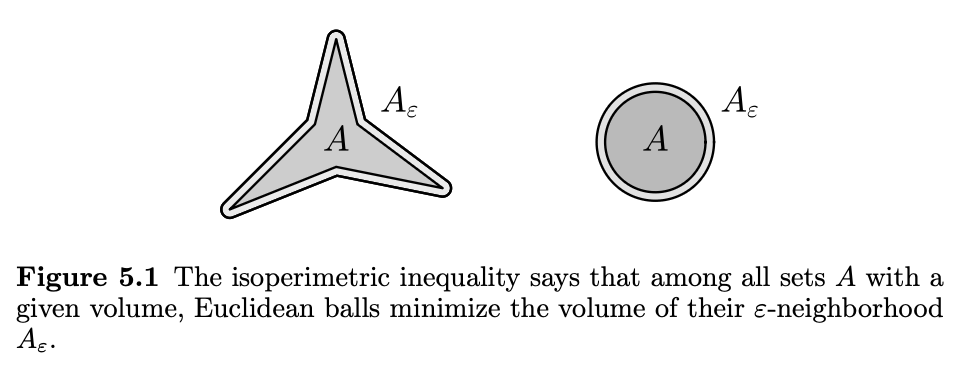
\includegraphics[width=0.8\textwidth]{Chapter 5/fig5-1.png}
\end{center}
\end{theorem}

A similar isoperimetric inequality holds for subsets on $S^{n - 1}$, and in this case the minimizers are the 
\underline{spherical caps} - neighborhoods of a single point. To state this principle, let $\sigma_{n - 1}$ 
denote the normalized are on the sphere $S^{n - 1}$ (The $n - 1$-dimensional Lebesgue measure).

\begin{theorem}[Isoperimetric inequality on the sphere]
\label{thm:5.1.5}
Let $\varepsilon > 0$. Then among all subsets $A \subset S^{n - 1}$ with given area $\sigma_{n - 1}(A)$, the 
spherical caps minimizer the area of the neighborhood $\sigma_{n - 1}(A_{\varepsilon})$, where 
\[ A_{\varepsilon} := \{ x \in \mathbb{R}^n: \ \exists y \in S^{n - 1} \text{ such that } 
\lVert x - y \rVert_{2} \leq \varepsilon \}. \]
\end{theorem}


\subsubsection{Blow-up of Sets on the Sphere}
The isoperimetric inequality leads to a remarkable and counterintuitive result: if a set $A$ covers at least 
half of the sphere in area, its $\varepsilon$-neighborhood $A_{\varepsilon}$ will cover most of the sphere. 
To simplify things in view of \cref{thm:5.1.3}, we'll operate on the sphere with radius $\sqrt{n}$.

\begin{lemma}[Blow-up]
\label{lem:5.1.6}
Let $A \subset \sqrt{n}S^{n - 1}$, and let $\sigma$ denote the normalized are on that sphere. If 
$\sigma(A) \geq 1/2$, then for every $t \geq 0$, 
\[ \sigma(A_t) \geq 1 - 2 \exp{(-ct^2)}. \]
\end{lemma}

\begin{proof}
Consider the hemisphere defined by the first coordinate:
\[ H := \{x \in \sqrt{n}S^{n - 1}: \ x_1 \leq 0 \}. \]
By assumption, $\sigma(A) \geq 1/2 = \sigma(H)$, hence the isoperimetric inequality (\cref{thm:5.1.5}) implies 
that 
\[ \sigma(A_t) \geq \sigma(H_t). \]
The neighborhood $H_t$ of the hemisphere $H$ is a spherical cap (a portion of a sphere cut off by a plane), 
and we could compute its area directly, but 
it is easier to use \cref{thm:3.4.5} instead, which states that a random vector $X \sim \mathrm{Unif}
(\sqrt{n}S^{n - 1})$ is subgaussian, and $\lVert X \rVert_{\psi_2} \leq C$. Since $\sigma$ is the uniform 
probability measure on the sphere, it follows that 
\[ \sigma(H_t) = P(X \in H_t). \]
Now, the definition of the neighborhood implies that 
\[ \{ x \in \sqrt{n}S^{n - 1}: \ x_1 \leq t / \sqrt{2} \} \subset H_t. \]
Thus
\[ \sigma(H_t) \geq P(X_1 \leq t / \sqrt{2}) \geq 1 - 2 \exp{(-ct^2)}. \]
The last inequality holds because $\lVert X_1 \rVert_{\psi_2} \leq \lVert X \rVert_{\psi_2} \leq C$. Then the 
lemma is proved because $\sigma(A_t) \geq \sigma(H_t)$.
\end{proof}

\begin{remark}[A more dramatic blow-up]
\label{rmk:5.1.7}
The $1/2$ value for the area in \cref{lem:5.1.6} was arbitrary, and can be replaced with any constant, or even 
an exponentially small quantity (Exercise 5.3)!
\end{remark}

\begin{remark}[A zero-one law]
\label{rmk:5.1.8}
The blow-up phenomenen we just saw can be quite counterintuitive at first. However, this is a typical p
phenomenon in high dimensions. It is similar to \textit{zero-one laws} in probability theory, which basically 
say that events influenced by many random variables tend to have probabilities zero or one.
\end{remark}


\subsubsection{Proof of Theorem 5.1.3}
WLOG, we can assume that $\lVert f \rVert_{\mathrm{Lip}} = 1$. Let $M$ denote the median of $f(X)$, which 
by definition satisfies 
\[ P(f(X) \leq M) \geq \frac{1}{2} \text{ and } P(f(X) \geq M) \geq \frac{1}{2}. \]
Consider the sublevel set 
\[ A := \{x \in \sqrt{n}S^{n - 1}: \ f(x) \leq M \}. \]
Since $P(X \in A) \geq \frac{1}{2}$, \cref{lem:5.1.6} implies that 
\[ P(X \in A_t) \geq 1 - 2 \exp{(-ct^2)}. \]
On the other hand, we claim that 
\[ P(X \in A_t) \leq P(f(X) \leq M + t). \]
Indeed, if $X \in A_t$ then $\lVert X - y \rVert_{2} \leq t$ for some point $y \in A$. By definition, 
$f(y) \leq M$. Since $f$ is Lipschitz with $\lVert f \rVert_{\mathrm{Lip}} = 1$, it follows that 
\[ f(X) \leq f(y) + \lVert X - y \rVert_{2} \leq M + t. \]
Combining the two bounds above, we conclude that 
\[ P(f(X) \leq M + t) \geq 1 - 2 \exp{(-ct^2)}. \]
Repeating the argument for $-f$, we obtain a similar bound for the probability that $f(x) \geq M - t$ (do). 
Combining the two, we get a similar bound for the probability that $|f(X) - M| \leq t$, and conclude that 
\[ \lVert f(X) - M \rVert_{\psi_2} \leq C. \]
Then we can replace the median by the mean, which follows by centering (\cref{lem:2.7.8}). Therefore the proof 
is complete. $\square$



% ----------5.2----------
\subsection{Concentration on Other Metric Measure Spaces}
We can extend concentration from the sphere to other spaces as well. The proof of \cref{thm:5.1.3} relied 
on two ingredients: 
\begin{enumerate}
	\item an isoperimetric inequality,
	\item a blow-up of its minimizers.
\end{enumerate}
There are not unique to the sphere - many spaces satusfy them hence we can derive similar concentration results.

\begin{remark}[]
\label{rmk:5.2.1}
Concentration keeps the mean, median, and $L^p$ norms close. Therefore, we can always replace the mean 
$\mathbb{E}[f(X)]$ with the median (Exercise 5.6), or, if the mean is nonnegative, with the $L^p$ norm for any 
$p \geq 1$, though the constant may depend on $p$ (Exercise 5.10).
\end{remark}


\subsubsection{Gaussian Concentration}
The \underline{Gaussian measure} of a Borel set $A \subset \mathbb{R}^n$ is defined as 
\[ \gamma_n(A) := P(X \in A) = \frac{1}{(2 \pi)^{n / 2}} \int_{A}^{} e^{-\lVert x \rVert_{2}^2 / 2} \ dx \]
where $X \sim N(0, I_n)$ is the standard normal random vector in $\mathbb{R}^n$.

\begin{theorem}[Gaussian isoperimetric inequality]
\label{thm:5.2.2}
Let $\varepsilon > 0$. Then among all sets $A \subset \mathbb{R}^n$ with given gaussian measure $\gamma_n(A)$, 
the half-spaces minimize the Gaussian measure of the neighborhood $\gamma_n(A_{\varepsilon})$.
\end{theorem}

\begin{theorem}[Gaussian concentration]
\label{thm:5.2.3}
Consider a random vector $X \sim N(0, I_n)$ and a Lipschitz function $f: \mathbb{R}^n \to \mathbb{R}$ (with 
respect to the Euclidean metric). Then 
\[ \lVert f(X) - \mathbb{E}[f(X)] \rVert_{\psi_2} \leq C \lVert f \rVert_{\mathrm{Lip}}. \]
\end{theorem}

\begin{example}[]
\label{ex:5.2.4}
Two special cases of \cref{thm:5.2.3} should already be familiar: 
\begin{enumerate}
	\item For linear functions $f$, it follows since $X \sim N(0, I_n)$ is subgaussian.
	\item For the Euclidean norm $f(x) = \lVert x \rVert_{2}$, it follows from norm concentration 
	(\cref{thm:3.1.1}).
\end{enumerate}
\end{example}


\subsubsection{Hamming Cube}
The method based on isoperimetry also works on the Hamming cube $(\{0, 1\}^n, d, \mathbb{P})$ 
(\cref{def:4.2.14}), where $d(x, y)$ is the normalized Hamming distance:
\[ d(x, y) = \frac{1}{n}|\{i: x_i \neq y_i\}|. \]
The measure $\mathbb{P}$ is the uniform probability measure on the cube: 
\[ \mathbb{P}(A) = \frac{|A|}{2^n} \text{ for any } A \subset \{0, 1\}^n. \]

\begin{theorem}[Concentration on the Hamming cube]
\label{ex:5.2.5}
Consider a random vector $X \sim \{0, 1\}^n$. Then for any function $f: \{0, 1\}^n \to \mathbb{R}$ we have 
\[ \lVert f(X) - \mathbb{E}[f(X)] \rVert_{\psi_2} \leq \frac{C \lVert f \rVert_{\mathrm{Lip}}}{\sqrt{n}}. \]
\end{theorem}


\subsubsection{Symmetric Group}
A similar result holds for the symmetric group $S_n$, a set of all $n!$ permutations of $\{1, \dots, n\}$. 
We can view the symmetric group as a metric measure space $(S_n, d, \mathbb{P})$, where $d(\pi, \rho)$ is the 
normalized Hamming distance - the fraction of the symbols on which permutations $\pi$ and $\rho$ differ:
\[ d(\pi, \rho) = \frac{1}{n} |\{i: \pi(i) \neq \rho(i)\}|. \]
The measure $\mathbb{P}$ is the uniform probability measure on $S_n$:
\[ \mathbb{P}(A) = \frac{|A|}{n!} \text{ for any } A \subset S_n. \]

\begin{theorem}[Concentration on the symmetric group]
\label{thm:5.2.6}
Consider a random permutation $X \sim \mathrm{Unif}(S_n)$ and a function $f: S_n \to \mathbb{R}$. Then 
\[ \lVert f(X) - \mathbb{E}[f(X)] \rVert_{\psi_2} \leq \frac{C \lVert f \rVert_{\mathrm{Lip}}}{\sqrt{n}}. \]
\end{theorem}


\subsubsection{Riemannian Manifolds with Strictly Positive Curvature}
(Feel free to skip this if not familiar with differential geometry)

A compact connected Riemannian manifold $(M, g)$ comes with the geodesic distance $d(x, y)$, which is the 
shortest length of a curve connecting the points. Then we can define a metric measure space $(M, d, \mathbb{P})$ 
where $\mathbb{P}$ is the uniform probability measure derived by normalizing the Riemannian volume. 

Let $c(M)$ denote the infimum of the Ricci curvature tensor over all tangent vectors. Assuming $c(M) > 0$, then 
it can be proved that 
\[ \lVert f(X) - \mathbb{E}[f(X)] \rVert_{\psi_2} \leq \frac{C \lVert f \rVert_{\mathrm{Lip}}}{\sqrt{c(M)}} \]
for any Lipschitz function $f: M \to \mathbb{R}$.

To give an example, $c(S^{n - 1}) = n - 1$. Then the above gives another approach for the concentration 
inequality of the sphere.


\subsubsection{Special Orthogonal Group}
The special orthogonal group $\mathrm{SO}(n)$ consists of all $n \times n$ orthogonal matrices with determinant 
1. We can treat it as a metric measure space $(\mathrm{SO}(n), \lVert \cdot \rVert_{F}, \mathbb{P})$, with 
distance given by the Frobenius norm $\lVert A - B \rVert_{F}$ and $\mathbb{P}$ as the uniform probability 
measure.

\begin{theorem}[Concentration on the special orthogonal group]
\label{thm:5.2.7}
Consider a random orthogonal matrix $X \sim \mathrm{Unif}(\mathrm{SO}(n))$ and a function $f: \mathrm{SO}(n) 
\to \mathbb{R}$. Then 
\[ \lVert f(X) - \mathbb{E}[f(X)] \rVert_{\psi_2} \leq \frac{C \lVert f \rVert_{\mathrm{Lip}}}{\sqrt{n}}. \]
\end{theorem}

The result above can be deduced from the concentration on general Riemannian manifolds.

\begin{remark}[Haar measure]
\label{rmk:5.2.8}
To generate a random orthogonal matrix $X \sim \mathrm{Unif}(\mathrm{SO}(n))$, one way is to start with an 
$n \times n$ Gaussian random matrix $G$ with $N(0, 1)$ independent entries, and compute its SVD 
$G = U \Omega V^T$. Then the matrix of left singular vectors is uniformly distributed in $\mathrm{SO}(n)$.

The uniform probability distribution on $\mathrm{SO}(n)$ is given by 
\[ \mu(A) := P(X \in A) \text{ for } A \subset \mathrm{SO}(n). \]
This is the unique rotation-invariant probaility measure on $\mathrm{SO}(n)$, called the 
\underline{Haar measure}.
\end{remark}


\subsubsection{Grassmannian}
The Grassmannian manifold $G_{n, m}$ consists of all $m$-dimensional subspaces of $\mathbb{R}^n$. When $m = 1$, 
it can be identified with the sphere $S^{n - 1}$. Therefore the concentration on the Grassmannian includes the 
concentration on the sphere. 

We can treat $G_{n, m}$ as a metric space $(G_{n, m}, d, \mathbb{P})$, where the distance between subspaces is 
given by the operator norm
\[ d(E, F) = \lVert P_E - P_F \rVert_{} \]
where $P_E$ and $P_F$ are the orthogonal projections onto the subspaces. The probability measure is the Haar 
measure (\cref{rmk:5.2.8}). A random subspace $E$ can hence be computed by computing the image of the random 
$n \times m$ Gaussian random matric with i.i.d. $N(0, 1)$ entries.

\begin{theorem}[Concentration on the Grassmannian]
\label{thm:5.2.9}
Consider a random subspace $X \sim \mathrm{Unif}(G_{n, m})$ and a function $f: G_{n, m} \to \mathbb{R}$. Then 
\[ \lVert f(X) - \mathbb{E}[f(X)] \rVert_{\psi_2} \leq \frac{C \lVert f \rVert_{\mathrm{Lip}}}{\sqrt{n}}. \]
\end{theorem}

\begin{proof}
The proof is a bit involved: Express the Grassmannian as the quotient via the special orthogonal group:
\[ G_{n, m} = \mathrm{SO}(n) / (\mathrm{SO}(m) \times \mathrm{SO}(n - m)) \]
and use the fact that concentration carries over to quotients.
\end{proof}


\subsubsection{Continuous Cube and Euclidean Ball}
\begin{theorem}[Concentration on the continuous cube and ball]
\label{thm:5.2.10}
Let $T$ be either the cube $[0, 1]^n$ or the ball $\sqrt{n}B_2^n$. Consider a random vector $X \sim 
\mathrm{Unif}(T)$ and a Lipschitz function $f; T \to \mathbb{R}$, where the Lipschitz norm is with respect 
to the Euclidean distance. Then 
\[ \lVert f(X) - \mathbb{E}[f(X)] \rVert_{\psi_2} \leq C \lVert f \rVert_{\mathrm{Lip}}. \]
\end{theorem}

\begin{proof}
Exercises 5.12 \& 5.13.
\end{proof}


\subsubsection{Densities of the Form \texorpdfstring{$e^{-U(x)}$}{}}
The push forward method from the previous section can be applied to many other distributions in $\mathbb{R}^n$. 
For example, suppose a random vector $X$ has a density of the form
\[ f(x) = e^{-U(x)} \]
for some function $U: \mathbb{R}^n \to \mathbb{R}$. For example, $X \sim N(0, I_n)$, the normal density gives 
$U(x) = \lVert x \rVert_{2}^2 + c$ where $c$ is constant (dependent on $n$ but not on $x$), and Gaussian 
concentration holds for $X$.

In general, we would expect that if $U$ has curvature at least like $\lVert x \rVert_{2}^2$, then there would be 
at least Gaussian concentration. As the theorem below shows, this depends on the Hessian of $U$:

\begin{theorem}[]
\label{thm:5.2.11}
Consider a random vector $X$ in $\mathbb{R}^n$ whose density has the form $e^{-U(x)}$ for some function 
$U: \mathbb{R}^n \to \mathbb{R}$. Assume there exists $\kappa > 0$ such that 
\[ \nabla^2 U(x) \succcurlyeq \kappa I_n \text{ for all } x \in \mathbb{R}^n. \]
Then any Lipschitz function $f: \mathbb{R}^n \to \mathbb{R}$ satisfies
\[ \lVert f(X) - \mathbb{E}[f(X)] \rVert_{\psi_2} \leq \frac{C \lVert f \rVert_{\mathrm{Lip}}}{\sqrt{\kappa}}. \]
\end{theorem}

\begin{proof}
THe proof uses semigroup methods, which are not covered in the text.
\end{proof}


\subsubsection{Random Vectors with Independent Bounded Coordinates}
There is a remarkable partial generalization of \cref{thm:5.2.10} for random vectors $X$ with independent 
coordinates that have arbitrary bounded distributions (not just uniform). By scaling, we can assume WLOG that 
$|X_i| \leq 1$.

\begin{theorem}[Talagrand concentration inequality]
\label{thm:5.2.12}
Consider a random vector in $\mathbb{R}^n$, 
$X = (X_1, \dots, X_n)$ whose coordinates are independent and satisfy $|X_i| \leq 1$ 
almost surely. Then for any Lipschitz function $f: [-1, 1]^n \to \mathbb{R}$, 
\[ \lVert f(X) - \mathbb{E}[f(X)] \rVert_{\psi_2} \leq C \lVert f \rVert_{\mathrm{Lip}}. \]
\end{theorem}



% ----------5.3----------
\subsection{Application: Johnson-Lindenstrauss Lemma}



% ----------5.4----------
\subsection{Matrix Bernstein Inequality}
We extend generalized concentration inequalities from sums of independent random variables to sums of 
independent random matrices. We'll make a matrix version of Bernstein inequality (\cref{thm:2.9.5}) by 
replacing random variables by random matrices, and absolute value by the operator norm. No need for 
independence of entries, rows, or columns within each random matrix!

\begin{theorem}[Matrix Bernstein inequality]
\label{thm:5.4.1}
Let $X_1, \dots, X_N$ be independent, mean zero, $n \times n$ symmetric random matrices, such that 
$\lVert X_i \rVert_{} \leq K$ almost surely for all $i$. Then for every $t \geq 0$, 
\[ P \left( \lVert \sum_{i = 1}^{N}X_i \rVert_{} \geq t \right) \leq 
2n \exp{\left( -\frac{t^2 / 2}{\sigma^2 + Kt / 3} \right)} \]
where $\sigma^2 = \lVert \sum_{i = 1}^{N} \mathbb{E}[X_i^2] \rVert_{}$ is the operator norm of the matrix 
variance of the sum.
\end{theorem}
We can rewrite the RHS of the inequality as the mixture of subgaussian and subexponential tail, like in the 
scalar Bernstein inequality:
\[ P \left( \lVert \sum_{i = 1}^{N}X_i \rVert_{} \geq t \right) \leq 
2n \exp{\left[ -c \cdot \min_{}\left( \frac{t^2}{\sigma^2}, \frac{t}{K} \right) \right]}. \]
The proof is similar to that of the scalar version: Repeat the MGF argument, swapping scalars with matrices. 
However, there is a big problem: Matrix multiplication is not commutative! Therefore we need some matrix 
calculus knowledge first.


\subsubsection{Matrix Calculus}
For an $n \times n$ symmetric matrix $X$, operations such as inversion or squaring only affect eigenvalues. 
For example, if the spectral decomposition of $X$ is $X = \sum_{i = 1}^{n} \lambda_i u_iu_i^T$, then
\[ X^{-1} = \sum_{i = 1}^{n} \frac{1}{\lambda_i}u_iu_i^T, \ 
X^2 = \sum_{i = 1}^{n} \lambda_i^2 u_iu_i^T, \ 
2I_n - 5X^3 = \sum_{i = 1}^{n} (2 - 5 \lambda_i^3)u_iu_i^T. \]
This suggest that for symmetric matrices, applying arbitrary functions on the matrices is equivalent to 
applying them to the eigenvalues:

\begin{definition}[Functions of matrices]
\label{def:5.4.2}
For a function $f: \mathbb{R} \to \mathbb{R}$ and an $n \times n$ symmetric matrix $X$ with spectral 
decomposition as above, define 
\[ f(X) := \sum_{i = 1}^{n} f(\lambda_i)u_iu_i^T. \]
\end{definition}
This definition agrees with matrix addition and multiplication, and with Taylor series (Exercise 5.16).

Of course, matrices can be compared with each other via a \underline{partial ordering}:
\begin{definition}[Loewner order]
\label{def:5.4.3}
We write $X \succcurlyeq 0$ if $X$ is a symmetric positive semidefinite matrix. We write $X \succeq Y$ and 
$Y \preceq X$ if $X - y \succeq 0$.
\end{definition}
This is a partial ordering because there are matrices for which neither $X \succeq Y$ nor $Y \succeq X$ holds.

\begin{proposition}[Simple properties of Loewner order]
\label{prop:5.4.4}
We have
\begin{enumerate}
	\item (Eigenvalue monotonicity) $X \preceq Y$ implies $\lambda_i(X) \leq \lambda_i(Y)$ for all $i$.
	\item (Trace monotonicity) For a (weakly) increasing function $f: \mathbb{R} \to \mathbb{R}$, 
	\[ X \preceq Y \implies \mathrm{tr}(f(X)) \leq \mathrm{tr}(f(Y)). \]
	\item (Operator norm) For any $a \geq 0$, 
	\[ \lVert X \rVert_{} \leq a \iff -aI_n \preceq X \preceq aI_n. \]
	\item (Upgrading scalar to matrix inequalities) For functions $f, g: \mathbb{R} \to \mathbb{R}$, 
	\[ f(x) \leq g(x) \forall x \text{ with } |x|\leq a \implies 
	f(X) \preceq g(X) \forall X \text{ with } \lVert X \rVert_{} \leq a. \]
\end{enumerate}
\end{proposition}

\begin{proof}
(a) If $X \preceq Y$, then $Y - X \succeq 0$ hence all eigenvalues of $Y - X$ are greater than equal to 0, 
and the result follows.

(b) The eigenvalues of $f(X)$ are $f(\lambda_i(X))$. The same can be said for $f(Y)$. By part (a) and the 
assumption, $f(\lambda_i(X)) \leq f(\lambda_i(Y))$. Summing these gives the result since the trace is the sum 
of the eigenvalues.

(c) From \cref{rmk:4.1.12}, $\lVert X \rVert_{} \leq a$ implies $u^T Xu \leq a$ for all unit vectors $u$. 
Therefore $u^T(aI_n - X)u \geq 0$ for all $u$, meaning $aI_n - X \succeq 0$, thus $X \preceq aI_n$. For the 
other inequality, again from \cref{rmk:4.1.12}, $u^T Xu \geq -a$ for all unit vectors $u$. Following the 
exact procedure above gives $X \succeq -aI_n$.

(d) By considering $g - f$, we can assume that $f = 0$. If $\lVert X \rVert_{} \leq a$, then all eigenvalues 
of $X$ satisfy $|\lambda_i| \leq a$, which implies $g(\lambda_i) \geq 0$ by assumption. So, by definition, 
$g(X)$ has nonnegative eigenvalues $g(\lambda_i)$ and so $g(X) \succeq 0$.
\end{proof}

\begin{remark}[Operator norm as matric absolute value]
\label{rmk:5.4.5}
(c) of \cref{prop:5.4.4} looks quite familiar... It is a matrix version of the basic fact about absolute 
values: for $x \in \mathbb{R}$, 
\[ |x| \leq a \iff -a \leq x \leq a. \]
This makes the operator norm $\lVert \cdot \rVert_{}$ a natural matrix version of the absolute value $|\cdot|$, 
and that's why it appeares in the matrix Bernstein inequality (\cref{thm:5.4.1}).
\end{remark}

\begin{remark}[Matrix monotonicity]
\label{rmk:5.4.6}
Can we strenghten trace monotonicity (\cref{prop:5.4.4} (b)) to matrix monotonicity, i.e.
\[ X \preceq Y \implies f(X) \preceq f(Y) \text{ for any weakly increasing } f: \mathbb{R} \to \mathbb{R}? \]
If $X$ and $Y$ commute, yes - but in general, no (Exercise 5.17). 

However, some functions, like $1/x$ and $\log_{}{x}$ on $[0, \infty)$, are \underline{matrix monotone}, meaning 
that the above holds even for non-commuting matrices:
\[ 0 \preceq X \preceq Y \implies X^{-1} \succeq Y^{-1} \succeq 0 \text{ and } \log_{}{X} \preceq \log_{}{Y} \]
whenever $X$ is invertible (Exercise 5.18).
\end{remark}


\subsubsection{Trace Inequalities}
Here is another identity that works for real numbers but not for matrices in general: $e^{x + y} = e^x e^y$ for 
scalars, but in Exercise 5.19, there are $n \times n$ symmetric matrices $X, Y$ such that 
\[ e^{X + Y} \neq e^X e^Y. \]
This is unfortunate, because when using the exponential moment method, we relied on this property to split 
the MGF via independence. 

Nevertheless, there are useful substitutes for the missing identity. In particular, this subsection covers two 
of them, both belonging to the rich family of \textit{trace inequalities}.

\begin{theorem}[Golden-Thompson inequality]
\label{thm:5.4.7}
For any $n \times n$ symmetric matrcies $A$ and $B$, 
\[ \mathrm{tr}(e^{A + B}) \leq \mathrm{tr}(e^A e^B). \]
\end{theorem}
Note that this does not hold for three or more matrices (we can find counterexamples)!

\begin{theorem}[Lieb inequality]
\label{thm:5.4.8}
Let $H$ be an $n \times n$ symmetric matrix. Define the function on matrices 
\[ f(X) := \mathrm{tr}(\exp{(H + \log_{}{X})}). \]
Then $f$ is concave on the space on PSD $n \times n$ symmetric matrices.
\end{theorem}

If $X$ is a random matrix, then Lieb and Jensen inequalities imply that 
\[ \mathbb{E}[f(X)] \leq f(\mathbb{E}[X]). \]
Applying this with $X = e^Z$, we obtain the following:

\begin{lemma}[Lieb inequality for random matrices]
\label{em:5.4.9}
Let $H$ be a fixed $n \times n$ symmetric matrix and $Z$ be a random $n \times n$ symmetric matrix. Then 
\[ \mathbb{E}[\mathrm{tr}(\exp{(H + Z)})] \leq \mathrm{tr}(\exp{(H + \log_{}{\mathbb{E}[e^Z]})}). \]
\end{lemma}


\subsubsection{Proof of Matrix Bernstein Inequality}



% ----------5.5----------
\subsection{Application: Community Detection in Sparse Networks}



% ----------5.6----------
\subsection{Application: Covariance Estimation for General Distributions}



% ----------5.7----------
\subsection{Extra notes}
There are lots of other concentration theorems not went over in the text. A very useful one is the McDiarmid 
inequality, which generalizes the Hoeffding inequality:

\begin{theorem}[McDiarmid inequality]
\label{thm:5.7.1}
Let $X = (X_1, \dots, X_N)$ be a random vector with independent entries. Let $f: \mathbb{R}^n \to \mathbb{R}$ 
be a measurable function. Assume that the value of $f(x)$ can change by at most $c_i > 0$ under an arbitrary 
change of a single coordinate of $x \in \mathbb{R}^n$. Then for any $t > 0$, 
\[ P(f(X) - \mathbb{E}[f(X)] \geq t) \leq \exp{\left( -\frac{2t^2}{\sum_{i = 1}^{N}c_i^2} \right)}. \]
\end{theorem}
